\documentclass[aspectratio=1610]{beamer}
\usepackage{theme}
% \usepackage[utf8x]{inputenc}

\usepackage[english]{babel}
\usepackage{calligra}
\usepackage{lmodern}
\usepackage{subcaption}
\usepackage{hyperref}

\usepackage{amsmath,amssymb,amsfonts,physics}
\usepackage{array, booktabs, makecell}
\usepackage{tabularx}

\usepackage{textcomp}
\makeatletter
\newcommand{\removelatexerror}{\let\@latex@error\@gobble}
\makeatother

% Graphics and video
\usepackage{graphicx,float,wrapfig}
\usepackage{animate}
\graphicspath{
  {./assets/images/}%
}


% args: big, bigg, Big, Bigg
\newcommand{\parenth}[2][]{#1(#2#1)}
\renewcommand{\bold}[1]{\textbf{\structure{#1}}}
  
\author[Daniotti \and Lucero]{Filippo Daniotti \and Taylor Lucero}
\title[NeRF-W]{\textsc{NeRF in the Wild}}
\subtitle{Neural Radiance Fields for Unconstrained Photo Collections}
\institute[DISI - UniTN]{Department of Information Engineering\\and Computer Science}
\date{\today}


\AtBeginSection[]
{
    \begin{frame}
        \frametitle{Contents}
        \tableofcontents[currentsection]
    \end{frame}
}

\begin{document}

\begin{frame}
    \titlepage
    \begin{figure}[H]
        \begin{center}
            
\includegraphics[width=0.4\linewidth]{marchio_unitrento_colore_it_202002.eps}
        \end{center}
    \end{figure}
\end{frame}


\begin{frame}
    \frametitle{Contents}
    \tableofcontents[sectionstyle=show,subsectionstyle=show,subsubsectionstyle=show/shaded/hide]
\end{frame}

\section{Introduction}
\begin{frame}{The problem: Novel view synthesis}
    We want to synthesize novel views of a scene from a sparse set of images  
    \bigskip
    \begin{figure}[H]
        % \animategraphics[loop,autoplay,width=.8\textwidth]{20}{assets/gifs/problem/problem-}{0}{57}
    \end{figure}
\end{frame}

\section{Background: Neural Radiance Fields (NeRF)}

\subsection{Core concepts}
\begin{frame}{Core concepts: representing a scene as a NeRF}
    \begin{block}{In a nutshell}
        NeRFs represent a continuous complex scene as a function 
        \begin{equation*}
            F_\theta : (\vb{x}, \vb{d}) \rightarrow (\vb{c}, \sigma)
        \end{equation*}
    \end{block}
    \begin{itemize}
        \item This function is approximated with a MLP \(F_\theta\)
        \begin{itemize}
            \item  overfitted to encode only scene!
        \end{itemize}
    \end{itemize}
    \bigskip
    \begin{figure}[H]
        \centering
        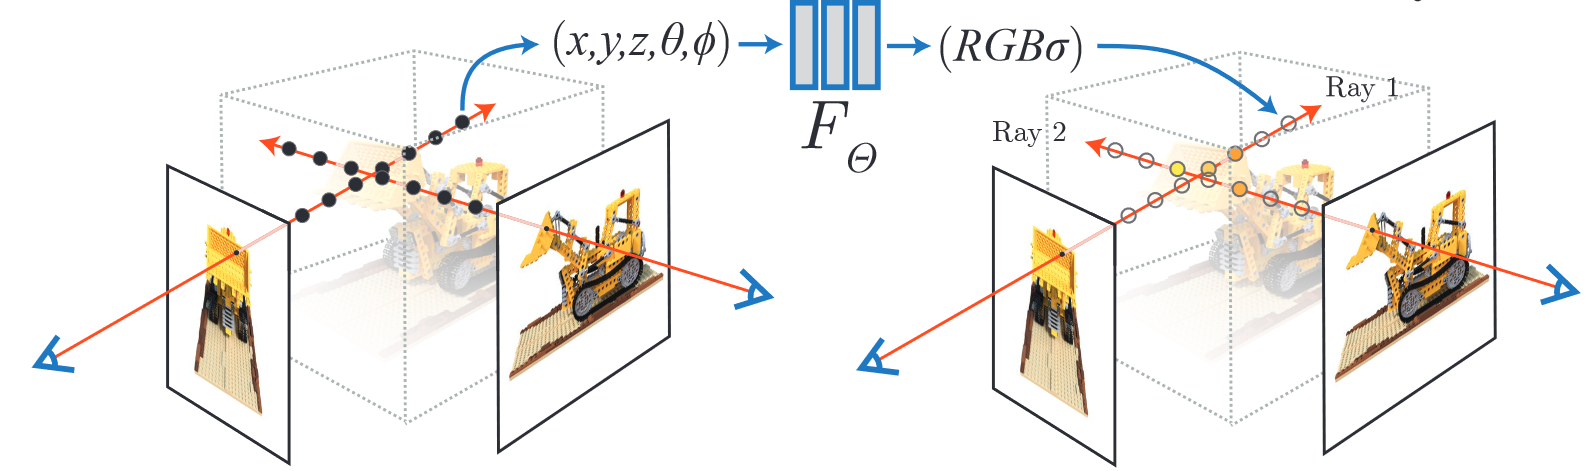
\includegraphics[width=.7\textwidth,keepaspectratio]{mapping}
    \end{figure}
\end{frame}

\begin{frame}{Core concepts: synthesizing novel views}
    \begin{columns}
        \begin{column}{.3\textwidth}
            \begin{figure}[H]
                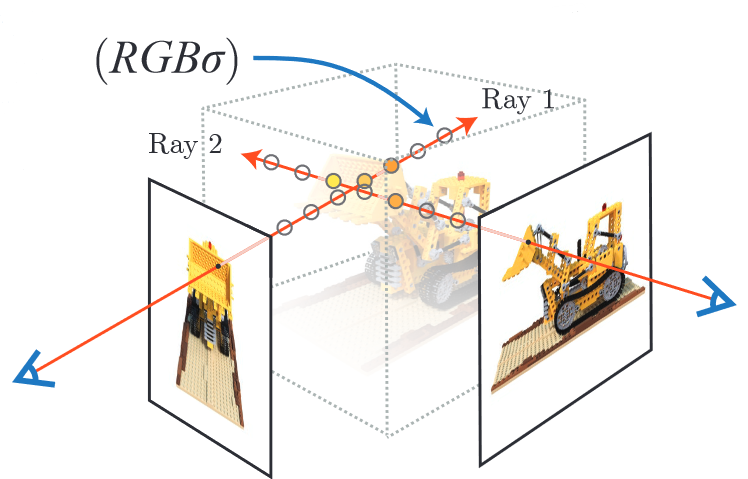
\includegraphics[width=\textwidth,keepaspectratio]{density-1}
            \end{figure}
        \end{column}
        \pause
        \begin{column}{.3\textwidth}
            \begin{figure}[H]
                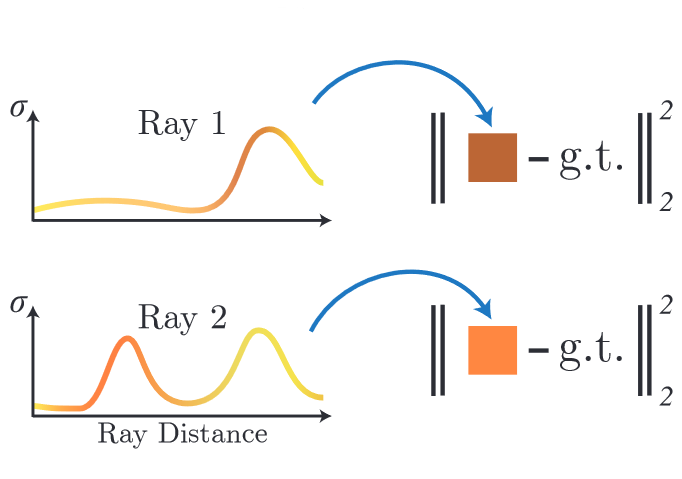
\includegraphics[width=\textwidth,keepaspectratio]{density-2}
            \end{figure}
        \end{column}
        \pause
        \begin{column}{.3\textwidth}
            \begin{figure}[H]
                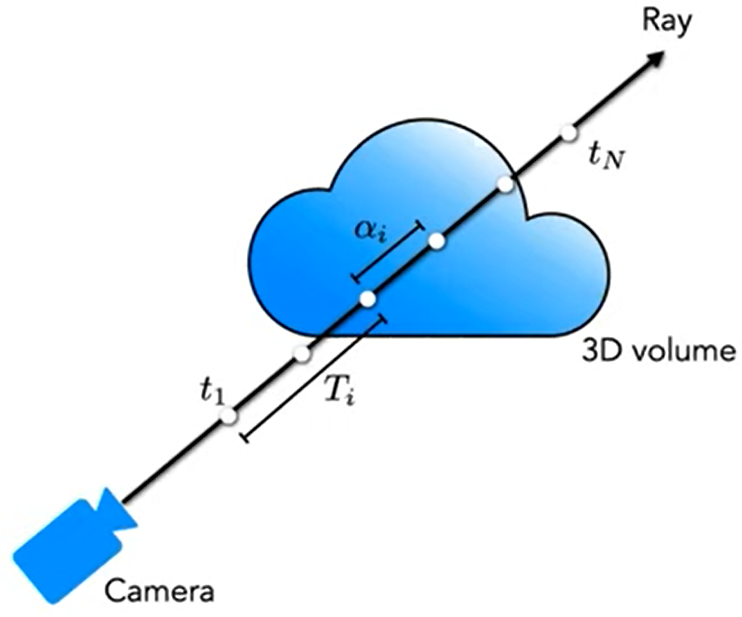
\includegraphics[width=\textwidth,keepaspectratio]{tracing}
            \end{figure}
        \end{column}
    \end{columns}
    \begin{onlyenv}<3->
        \begin{block}{Volume rendering with Radiance Fields} 
            Approximate the expected color \(\hat{\vb{C}}(\vb{r})\) encountered by camera ray \(\vb{r}(t) = \vb{o} + t\vb{d}\)
            \begin{equation*}
                \hat{\vb{C}}(\vb{r}) = \mathcal{R}(\vb{r}, \vb{c}, \sigma) = \sum_{k = 1}^{K} T(t_k) \alpha (\sigma (t_k)\delta_k) \vb{c}(t_k)
            \end{equation*}
        \end{block}
    \end{onlyenv}
\end{frame}

\subsection{Model}
\begin{frame}{Architecture}
    \begin{onlyenv}<1>
        \begin{figure}[H]
            \centering
            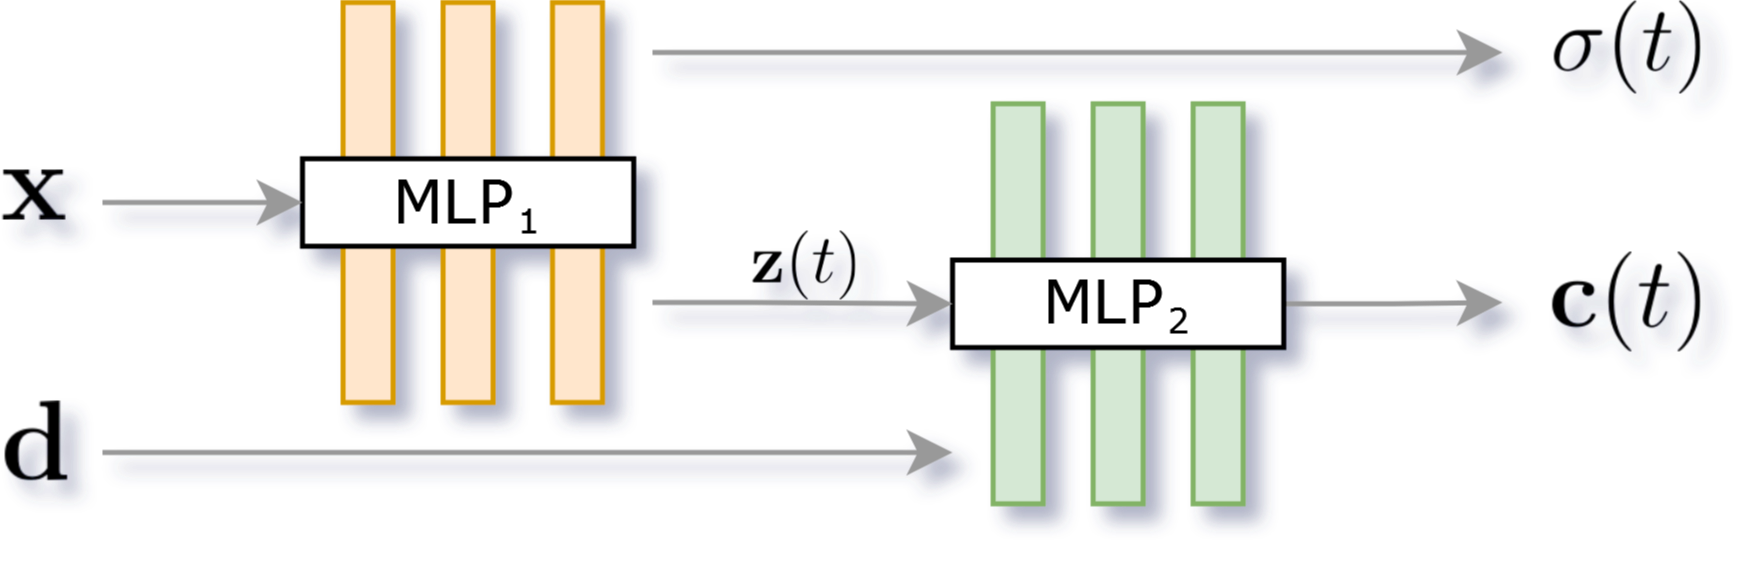
\includegraphics[width=.8\textwidth]{nerf-architecture}
        \end{figure}
    \end{onlyenv}

    \pause
    
    \begin{onlyenv}<2->
        \begin{columns}
            \begin{column}{.7\textwidth}
                \begin{figure}[H]
                    \centering
                    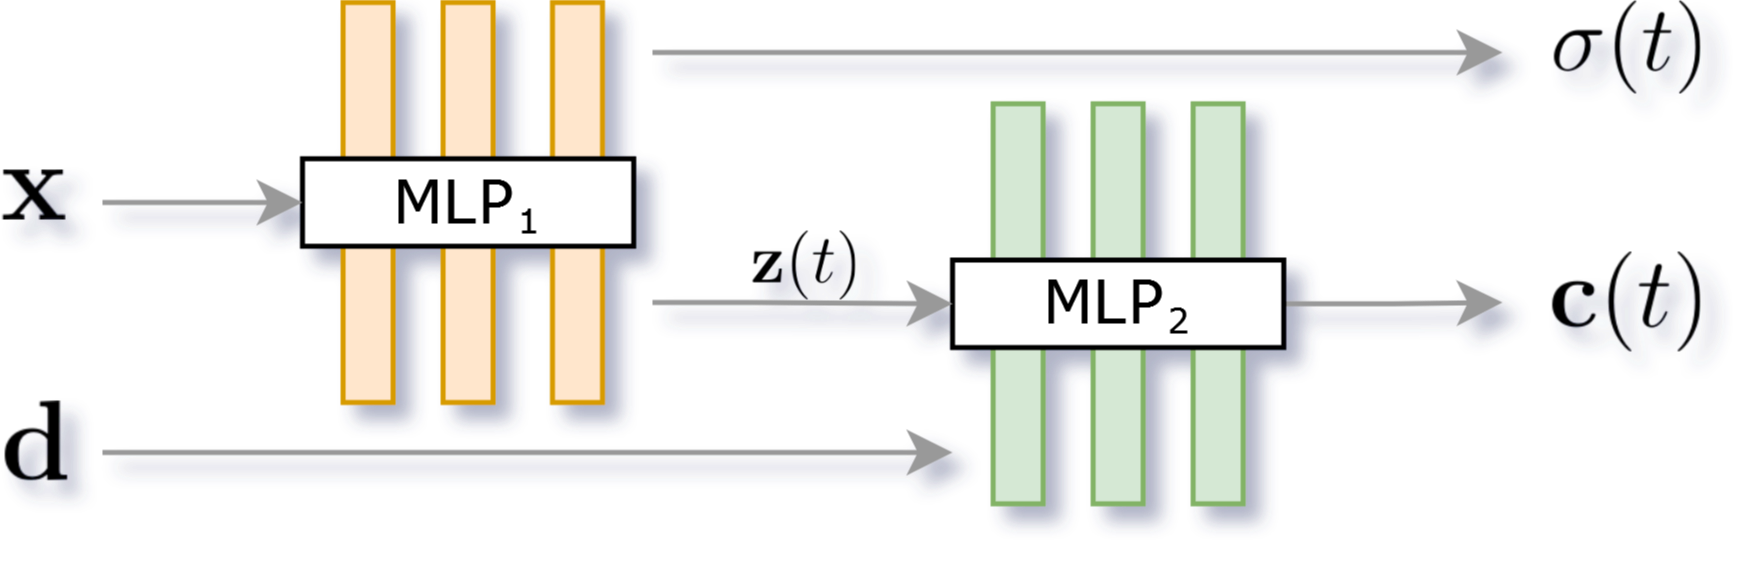
\includegraphics[width=.65\textwidth]{nerf-architecture}
                \end{figure}
            \end{column}
            \begin{column}{.3\textwidth}
                \Large{Why?}
            \end{column}
        \end{columns}
        \vspace{1.2cm}

        \pause

        \uncover<3->{
            \begin{columns}
                \begin{column}{.3\textwidth}
                    \centering
                    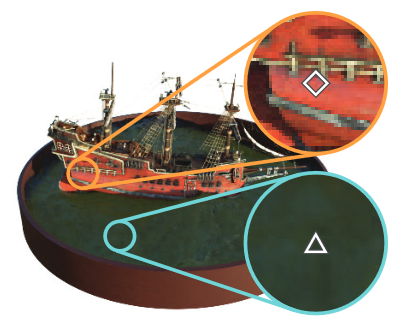
\includegraphics[width=.75\textwidth]{architecture-why-1.png}
                \end{column}
                \pause
                \begin{column}{.3\textwidth}
                    \centering
                    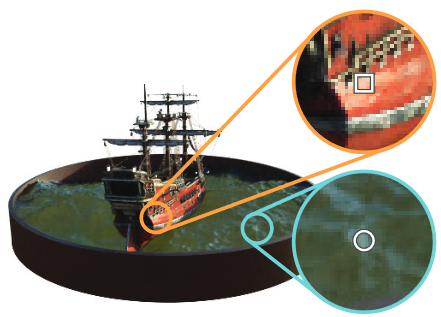
\includegraphics[width=.75\textwidth]{architecture-why-2.png}
                \end{column}
                \pause
                \begin{column}{.3\textwidth}
                    \centering
                    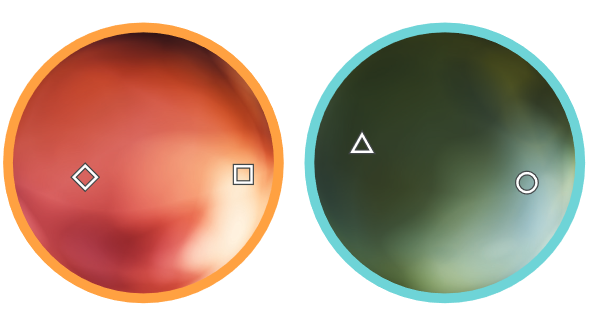
\includegraphics[width=.9\textwidth]{architecture-why-3.png}
                \end{column}
            \end{columns}
        }
    \end{onlyenv}
\end{frame}

\begin{frame}{Optimizing NeRFs}
    A few tricks are employed
    \bigskip
    \begin{columns}[t]
        \begin{column}{.42\textwidth}
            \bold{Positional encoding}\footnotemark\\
            map \(\vb{x}\), \(\vb{d}\) to a higher-dimensional space
            \begin{align*}
                [\sigma(t), \vb{z}(t)] & = \textrm{MLP}_{\theta_1} (\alert<2>{\gamma}_{\vb{x}}(\vb{x})) \\
                \vb{c}(t) & = \textrm{MLP}_{\theta_2} (\vb{z}(t), \alert<2>{\gamma}_{\vb{d}}(\vb{d}))
            \end{align*}
        \end{column}
        \begin{column}{.42\textwidth}
            \bold{Hierarchical volume sampling}\\
            use 2 MLPs sequentially
            \begin{align*}
                &\vb{\hat{C}}^c(\vb{r}) \rightarrow \textrm{coarse one}\\
                &\vb{\hat{C}}^f(\vb{r}) \rightarrow \textrm{fine one}
            \end{align*}
        \end{column}
    \end{columns}
    \bigskip
    \pause
    \begin{block}{Positional encoding}
        \begin{equation*}
            \gamma (\vb{x}) = \parenth[\bigg] {\sin (2^i \pi \vb{x}), \cos (2^i \pi \vb{x})}, \quad \forall i, 0 \le i \le L
        \end{equation*}
    \end{block}
    \footnotetext[1]{Tancik et al. 2020, \emph{Fourier Features Let Networks Learn High Frequency Functions in Low Dimensional Domains}, \url{https://arxiv.org/abs/2006.10739}}
\end{frame}

\begin{frame}{Optimizing NeRFs}
    \begin{columns}
        \begin{column}{.5\textwidth}
            \begin{figure}
                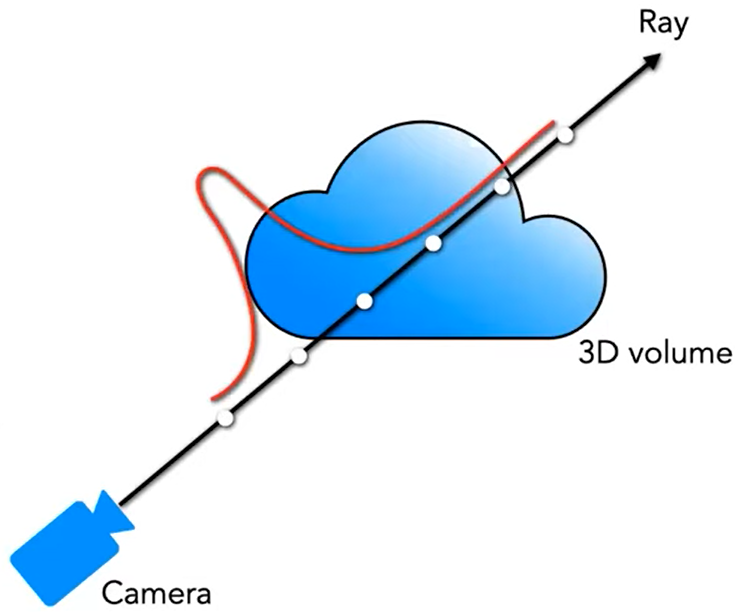
\includegraphics[width=.7\textwidth]{coarse.png}
            \end{figure}
        \end{column}
        \begin{column}{.5\textwidth}
            \begin{figure}
                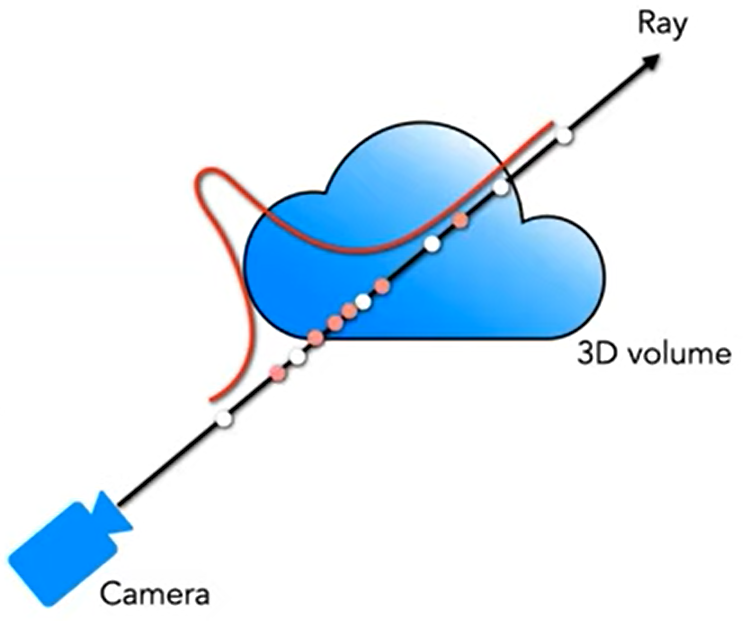
\includegraphics[width=.7\textwidth]{coarse-fine.png}
            \end{figure}
        \end{column}
    \end{columns}
    \bigskip
    \begin{block}{Training objective}
        \begin{equation}
            \sum_{\vb{r} \in \mathcal{R}} ||\vb{C}(\vb{r}) - \vb{\hat{C}}^c(\vb{r})||_2^2 + ||\vb{C}(\vb{r}) - \vb{\hat{C}}^f(\vb{r})||_2^2
        \end{equation}
    \end{block}
\end{frame}

\begin{frame}{NeRF Limitations}
    \begin{itemize}
        \item NeRFs assume real world scenes to be \bold{static}
        \pause
        \begin{itemize}
            \item this is often not the case!
        \end{itemize}
    \end{itemize}
    \vspace{1.2cm}
    \begin{columns}[t]
        \begin{column}{.4\textwidth}
            Photometric variations\\
        \end{column}
        \begin{column}{.4\textwidth}
            Transient objects\\
        \end{column}
    \end{columns}
    \begin{columns}
        \begin{column}{.4\textwidth}
            \begin{center}
                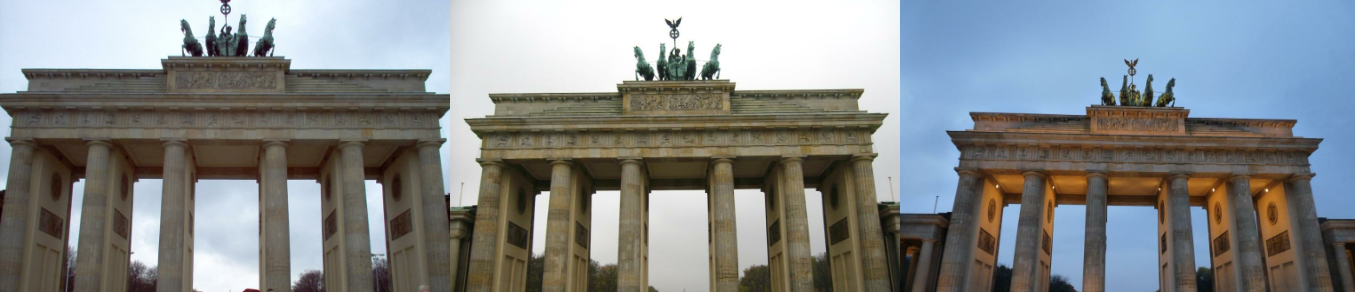
\includegraphics[width=\textwidth]{issues-var.png}
            \end{center}
        \end{column}
        \begin{column}{.4\textwidth}
            \begin{center}
                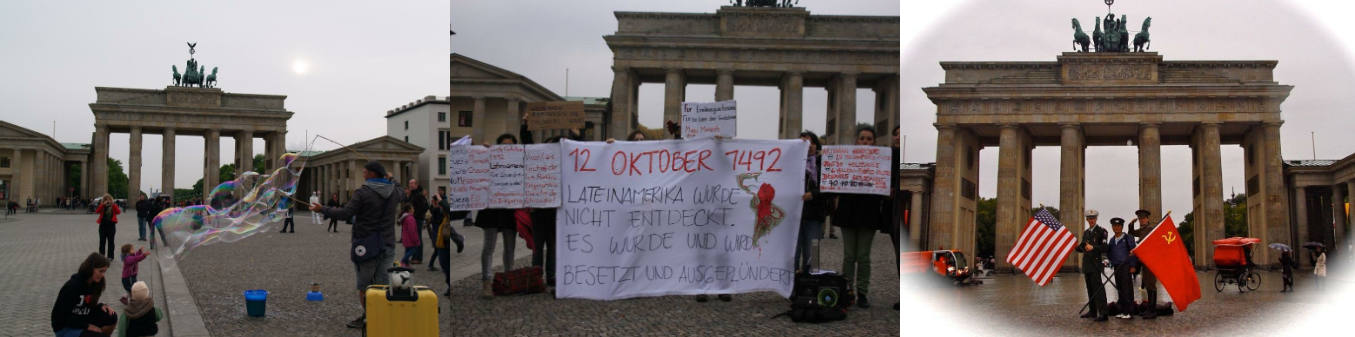
\includegraphics[width=\textwidth]{issues-transient.png}
            \end{center}
        \end{column}
    \end{columns}
    \vspace{1.2cm}
    \pause
    NeRF in the wild addresses these two issues
\end{frame}

\section{NeRF in the Wild (NeRF-W)}

\subsection{Latent appearence modeling}
\begin{frame}{Latent appearence modeling}
    \begin{block}{Generative Latent Optimization}
        Assign a \(\ell_i^{(a)}\) 
        appearence embedding vector to each image \(\mathcal{I}_i\)
        \begin{equation*}
            \vb{c}_i(t) = \textrm{MLP}_{\theta_2} (\vb{z}(t), \gamma_{\vb{d}}(\vb{d}), \alert{\ell_i^{(a)}})
        \end{equation*}
    \end{block}
    \begin{onlyenv}<2>
        \bigskip
        \begin{figure}[H]
            \centering
            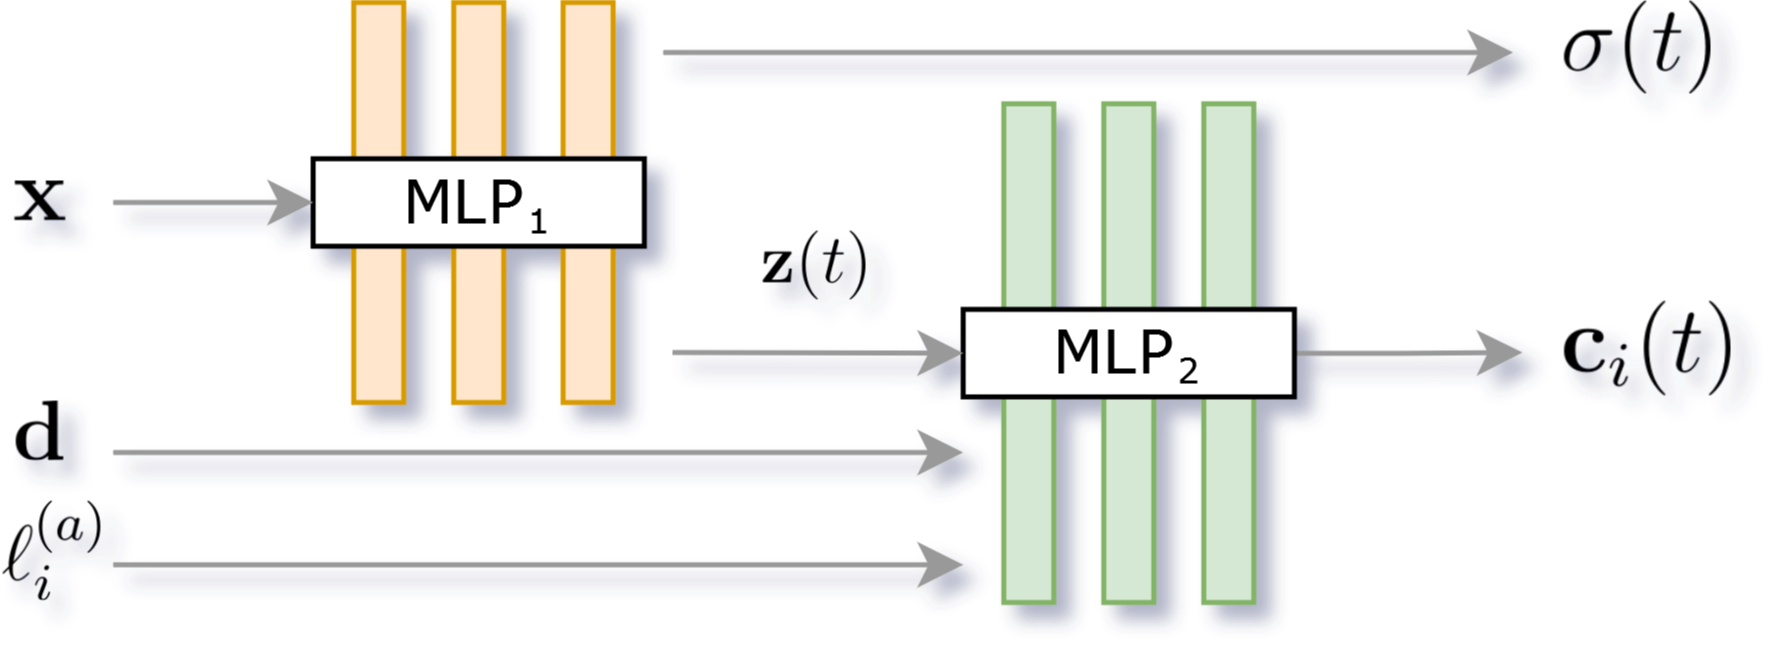
\includegraphics[width=.65\textwidth,keepaspectratio]{nerfa-architecture.png}
        \end{figure}
    \end{onlyenv}
\end{frame}

\begin{frame}{The appearence embedding vector}
    \begin{itemize}
        \item \(\ell_i^{(a)}\) fed only to MLP\(_{\theta_2}\) 
        \begin{itemize}
            \item keep 3D geometry prediction static
            \item modulate emitted radiance and ensure smooth interpolation
        \end{itemize} 
    \end{itemize}
    \bigskip
    \begin{figure}[H]
        \centering
        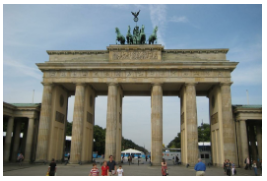
\includegraphics[width=.2\textwidth,keepaspectratio]{nerfa-results-1.png}
        \hspace{4cm}
        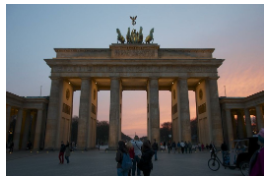
\includegraphics[width=.2\textwidth,keepaspectratio]{nerfa-results-3.png}\\
        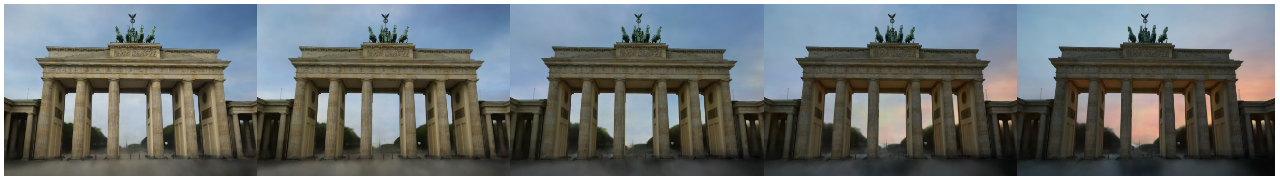
\includegraphics[width=.9\textwidth,keepaspectratio]{nerfa-results-2.png}
    \end{figure}
\end{frame}

\subsection{Transient component}
\begin{frame}{Transient Head}
    Transient phenomena alter both radiance and image density
    \bigskip
    \begin{center}
        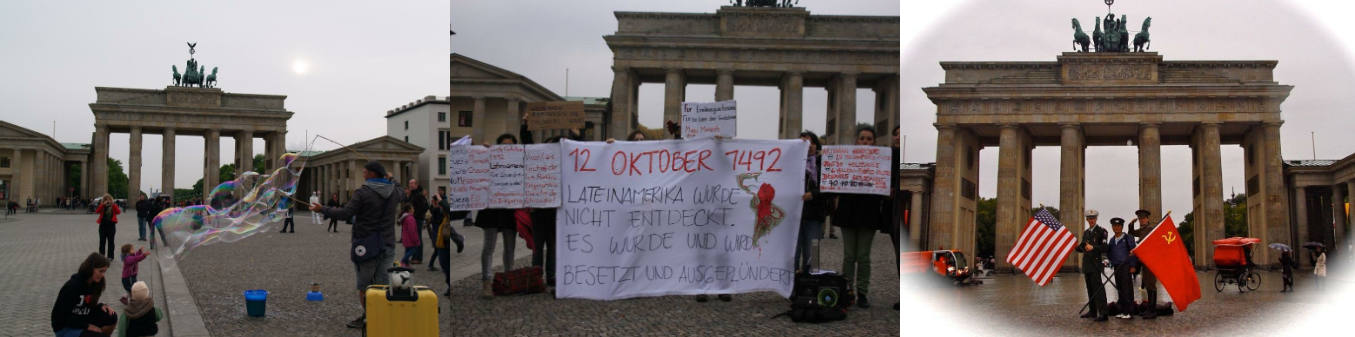
\includegraphics[width=.5\textwidth]{issues-transient.png}
    \end{center}
    \bigskip
    \pause
    \begin{columns}
        \begin{column}{.5\textwidth}
            \begin{onlyenv}<2->
                \begin{itemize}
                    \item we need a way to disentangle static vs. transient representation of the scene
                    \begin{itemize}
                        \item add a separate MLP head
                    \end{itemize}
                \end{itemize}
            \end{onlyenv}
            \uncover<3->{
                \begin{itemize}
                    \item transient representation should be image-dependent
                    \begin{itemize}
                        \item use a transient embedding vector \(\ell_i^{(\tau)}\)
                    \end{itemize}
                \end{itemize}
            }
        \end{column}
        \begin{column}{.5\textwidth}
            \begin{onlyenv}<2>
                \begin{center}
                    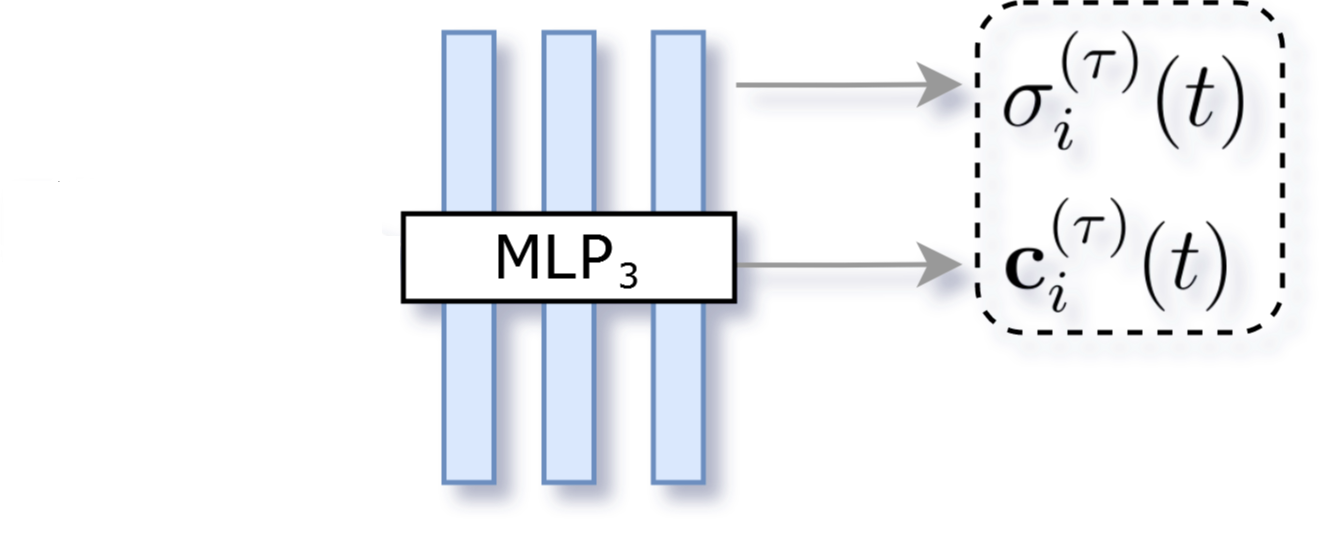
\includegraphics[width=.9\textwidth]{nerfu-no-t.png}
                \end{center}
            \end{onlyenv}
            \begin{onlyenv}<3->
                \begin{center}
                    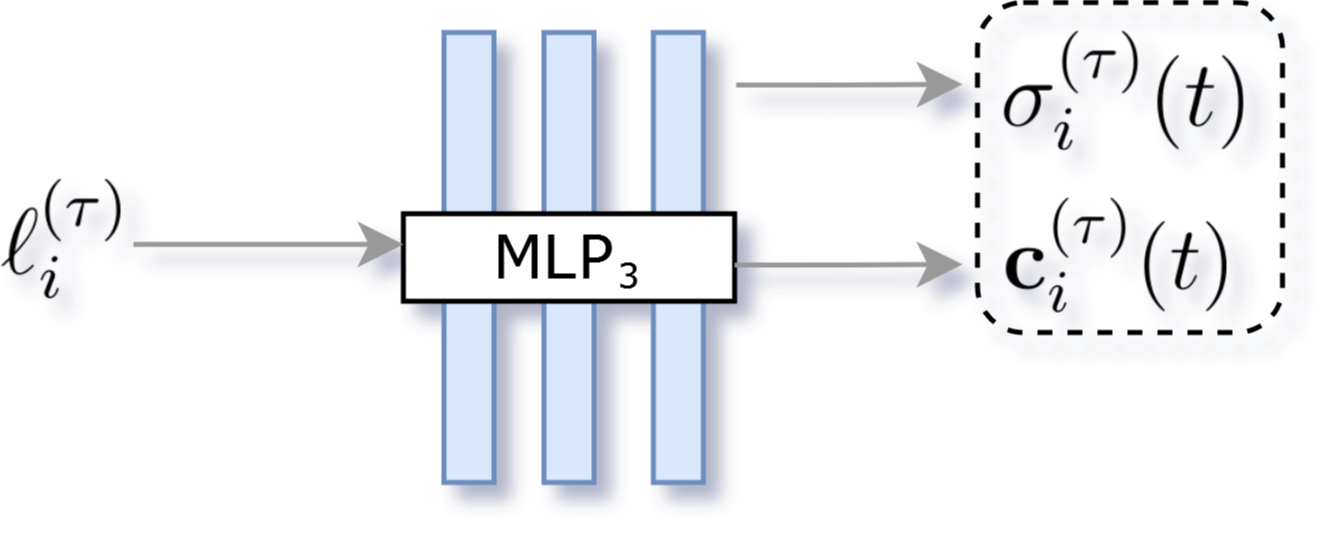
\includegraphics[width=.9\textwidth]{nerfu-t.png}
                \end{center}
            \end{onlyenv}
        \end{column}
    \end{columns}
\end{frame}

\begin{frame}{Rendering}
    \begin{block}{NeRF-W volume rendering}
        \begin{equation*}
            \hat{\vb{C}}(\vb{r}) = \sum_{k = 1}^{K} T(t_k) ( \alpha (\sigma (t_k)\delta_k)  \vb{c}(t_k)  \alert<1>{+ (\sigma_i^{(\tau)} (t_k)\delta_k)  \vb{c}_i^{(\tau)}(t_k)})
        \end{equation*}
    \end{block}
    \bigskip
    \pause
    \begin{figure}[H]
        \centering
        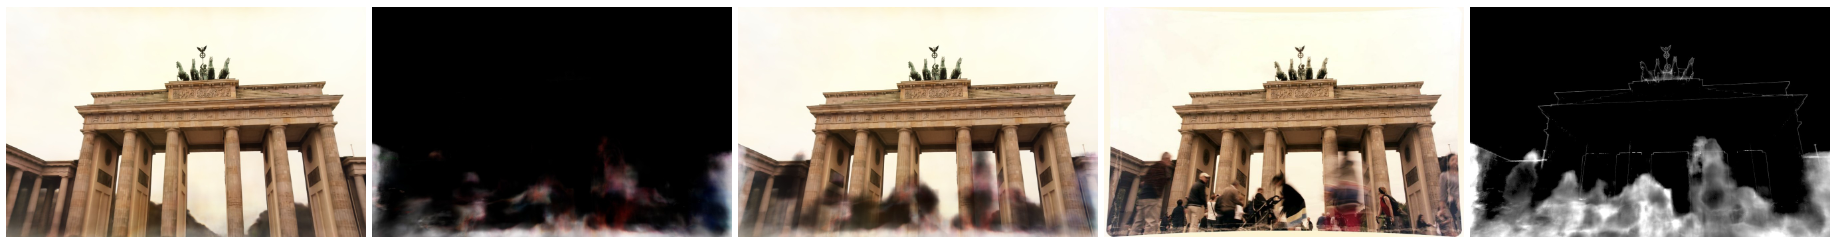
\includegraphics[width=.75\textwidth]{render.png}
    \end{figure}
\end{frame}

\begin{frame}{Uncertainty field}
    But... 
    \pause
    \begin{itemize}
        \item not all pixels are equally reliable
        \begin{itemize}
            \item learn a \emph{uncertainty field} \(\beta_i\)
            \item adapt reconstruction loss to ignore unreliable pixels and 3D locations likely to contain occluders
            \item actual color is modeled as a normal distribution with \(\beta_i\) as variance
        \end{itemize}
    \end{itemize}
    \bigskip
    \pause
    \begin{figure}[H]
        \centering
        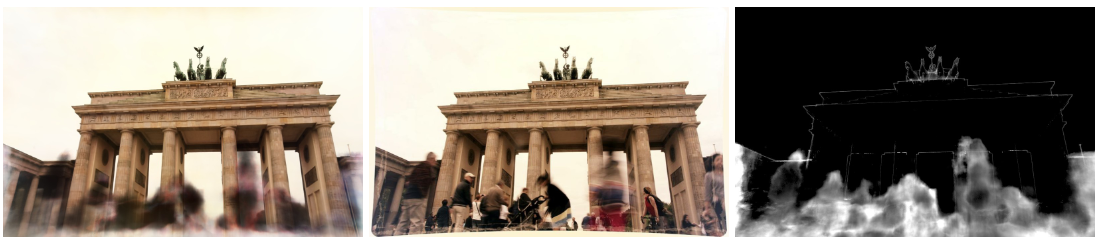
\includegraphics[width=.75\textwidth]{uncertainty.png}
    \end{figure}
    \bigskip
    \pause
    \begin{equation*}
        \bigg[\sigma_i^{(\tau)} (t), \vb{c}_i^{(\tau)} (t), \tilde{\beta}_i (t)\bigg] = \textrm{MLP}_{\theta_3} \parenth[\bigg]{\vb{z}(t), \ell_i^{(\tau)}},
        \quad\quad 
        \beta_i (t) = \beta_{\textrm{min}} + \textrm{softplus}\parenth[\bigg]{\tilde{\beta}_i (t)}
    \end{equation*}
\end{frame}

\begin{frame}{NeRF-W full architecture}
    \begin{onlyenv}<1>
        \begin{figure}[H]
            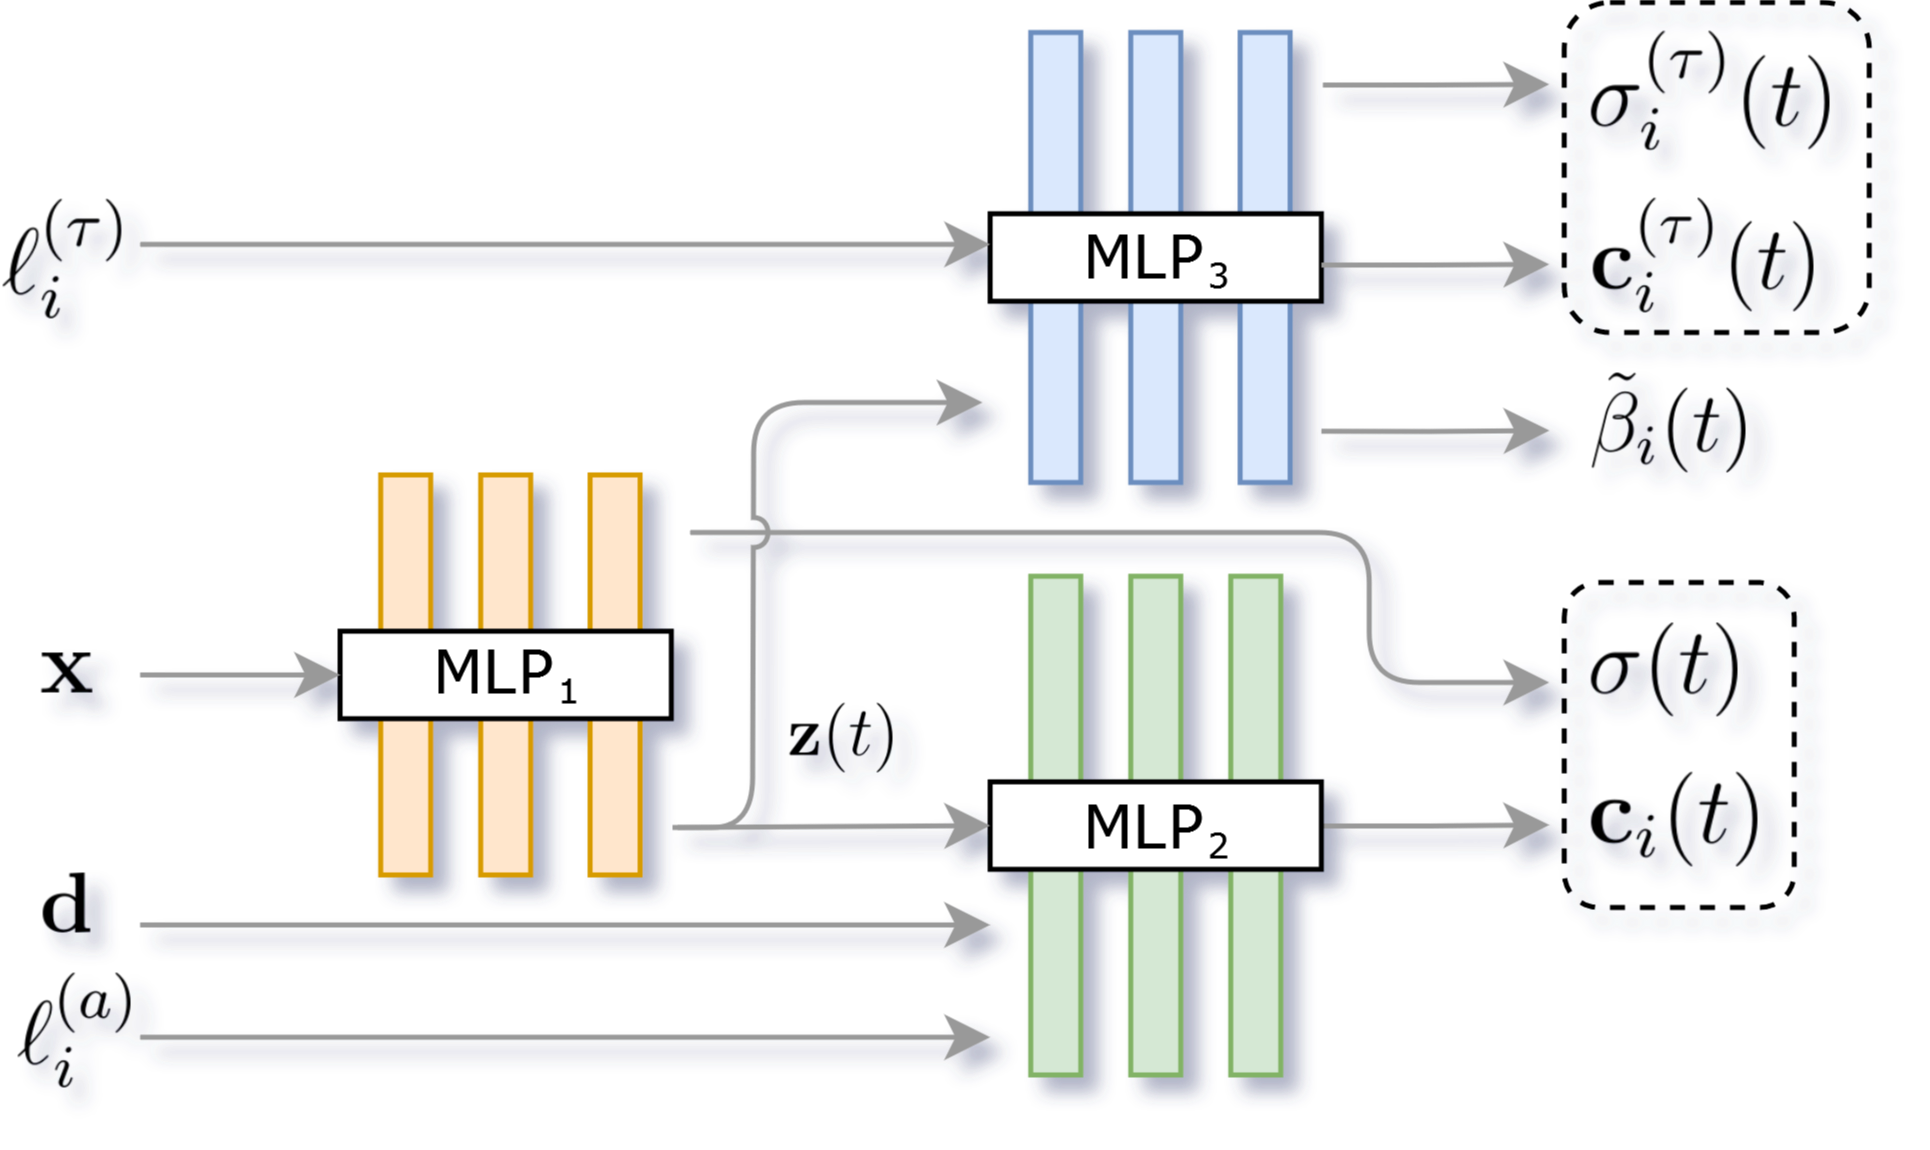
\includegraphics[width=.8\textwidth,keepaspectratio]{nerfw-architecture.png}
        \end{figure}
    \end{onlyenv}
    \begin{onlyenv}<2>
        \begin{columns}
            \begin{column}{.7\textwidth}
                \begin{figure}[H]
                    \raggedleft
                    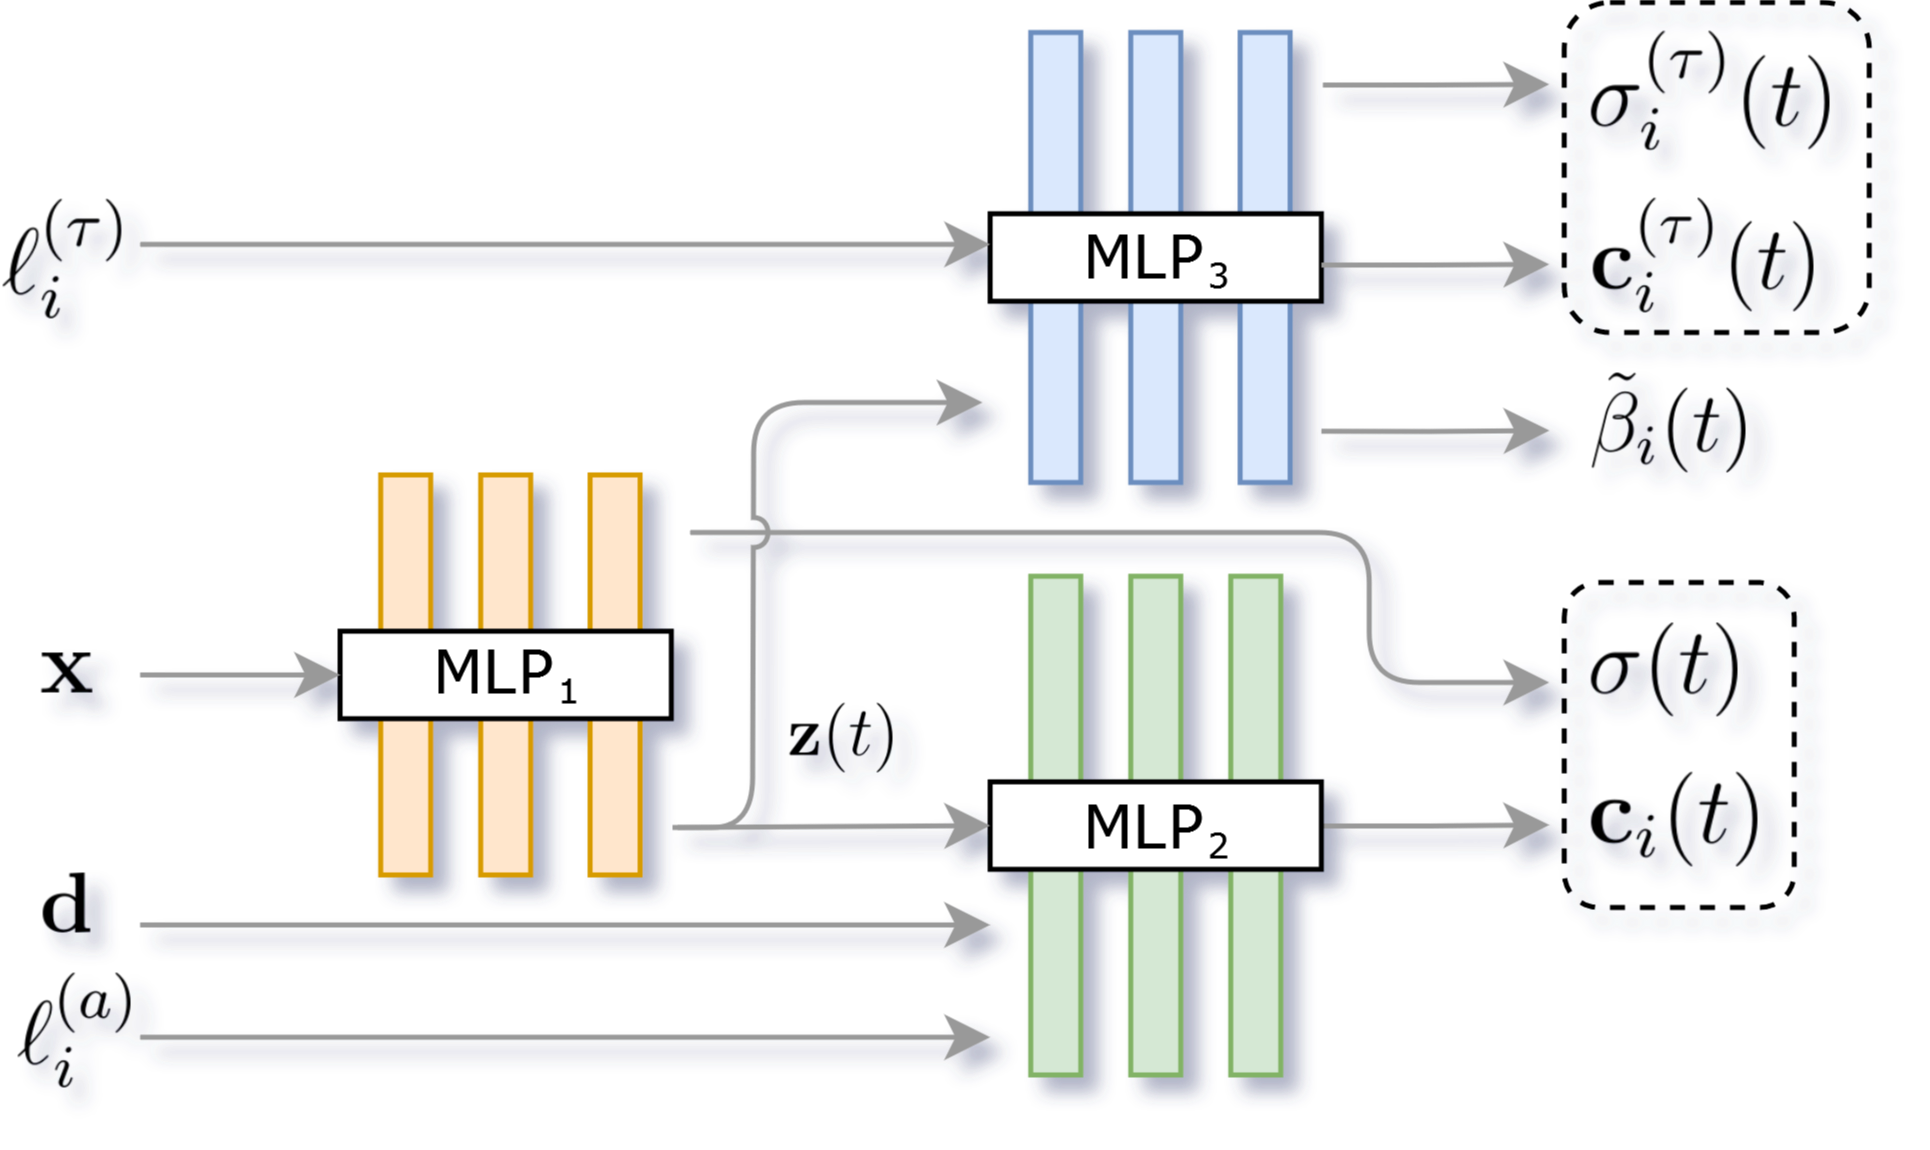
\includegraphics[width=.9\textwidth,keepaspectratio]{nerfw-architecture.png}
                \end{figure}
            \end{column}
            \begin{column}{.3\textwidth}
                \begin{itemize}
                    \item MLP\(_1\)
                    \begin{itemize}
                        \item 8 hidden layers
                        \item 512 units each
                    \end{itemize}
                    \item MLP\(_2\) and MLP\(_3\)
                    \begin{itemize}
                        \item 4 hidden layers
                        \item 128 units each
                    \end{itemize}
                \end{itemize}
            \end{column}
        \end{columns}

    \end{onlyenv}
\end{frame}

\subsection{Optimizing NeRF-W}
\begin{frame}{Optimization}
    \begin{block}{Objective}
        \begin{itemize}
            \item Fine model: loss for ray \(\vb{r}\) in image \(i\) with true color \(\vb{C}(\vb{r})\)
            \begin{equation*}
                L_i(\vb{r}) 
                = \frac{|| \vb{C}_i (\vb{r}) - \hat{\vb{C}}_i (\vb{r}) ||_2^2}{2\beta_i (\vb{r})^2} 
                + \frac{\log \beta_i (\vb{r})^2}{2} 
                + \frac{\lambda_u}{K} \sum^K_{k=1}\sigma_i^{(\tau)} (t_k)
            \end{equation*}
            \item Coarse model: only uses latent appearance modeling component
            \begin{equation*}
                \sum_{ij} L_i (\vb{r}_{ij}) + \frac{1}{2} || \vb{C} (\vb{r}_{ij}) - \hat{\vb{C}}_i^c (\vb{r}_{ij}) ||^2_2 
            \end{equation*}
            \item hyperparameters: \(n_i^{(a)}\), \(n_i^{(\tau)}\), \(\beta_{\textrm{min}}\), \(\lambda_u\)
        \end{itemize}
    \end{block}  
\end{frame}

\subsection{Results and ablation study}
\begin{frame}{Results: interpolations}
    \begin{figure}[H]
        % \animategraphics[loop,autoplay,width=.7\textwidth]{60}{assets/gifs/interpol/interpol-}{0}{449}
    \end{figure}
\end{frame}
\begin{frame}{Results: consistent geometry}
    \begin{figure}[H]
        % \animategraphics[loop,autoplay,width=.7\textwidth]{60}{assets/gifs/geometry/geometry-}{0}{209}
    \end{figure}
\end{frame}
\begin{frame}{Results}
    \begin{center}
        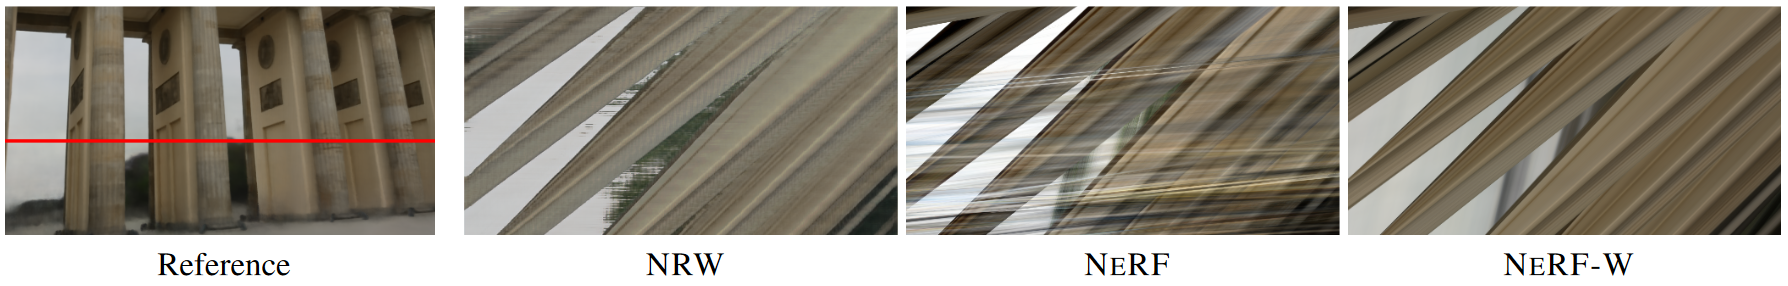
\includegraphics[width=\textwidth]{epipolar.png}
    \end{center}
    \bigskip
    \pause
    \begin{center}
        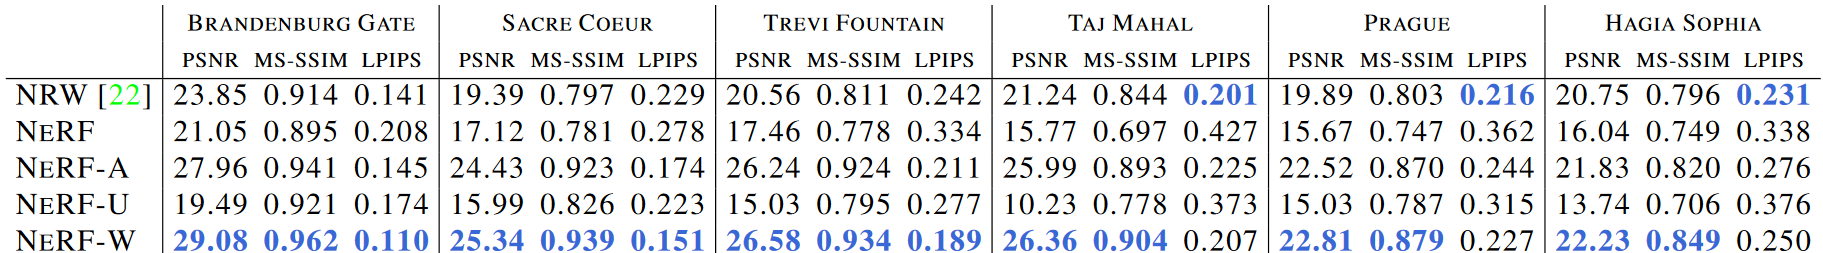
\includegraphics[width=\textwidth]{table.png}
    \end{center}
\end{frame}
\begin{frame}{Ablation study: Phototourism dataset}
    \begin{center}
        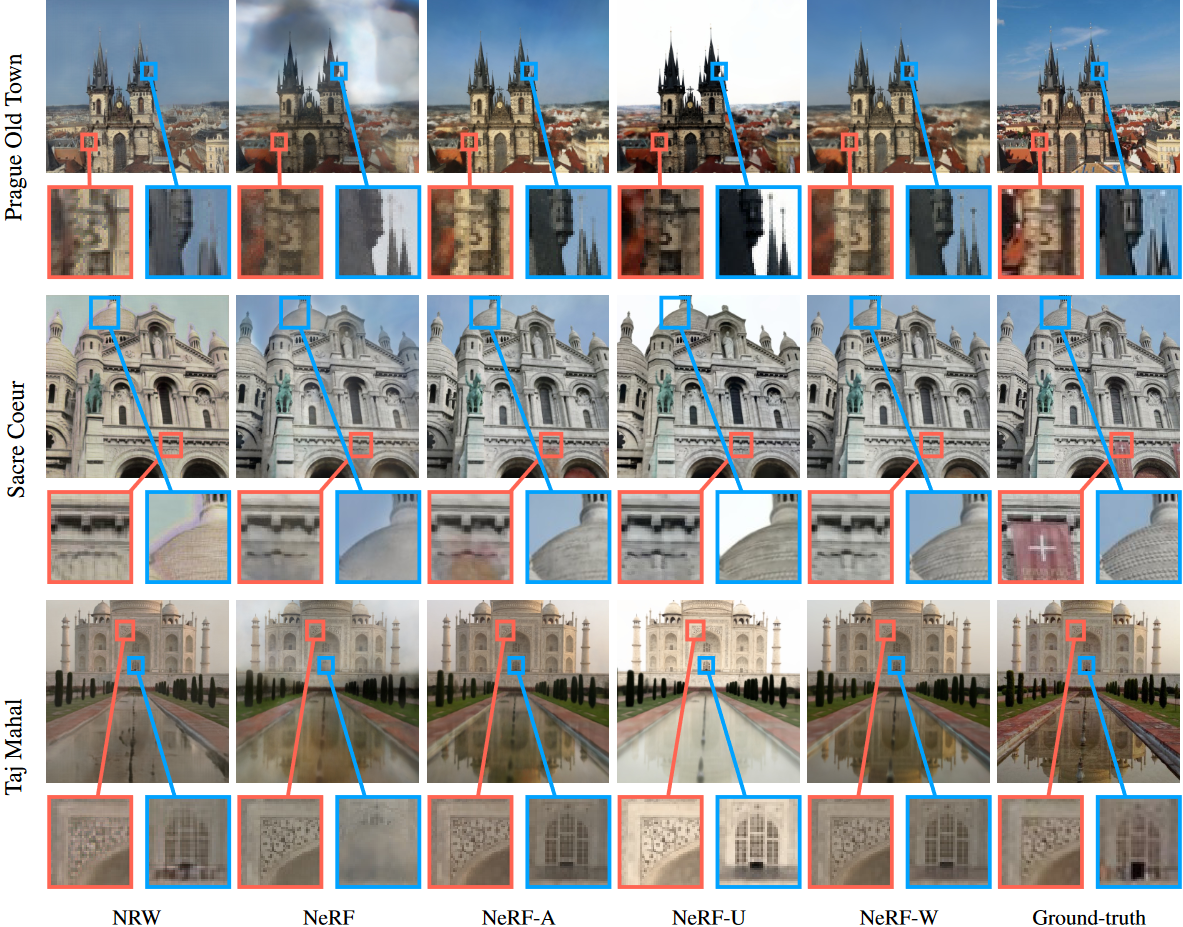
\includegraphics[width=.69\textwidth]{res-photo.png}
    \end{center}
\end{frame}
\begin{frame}{Ablation study: Lego dataset}
    \begin{center}
        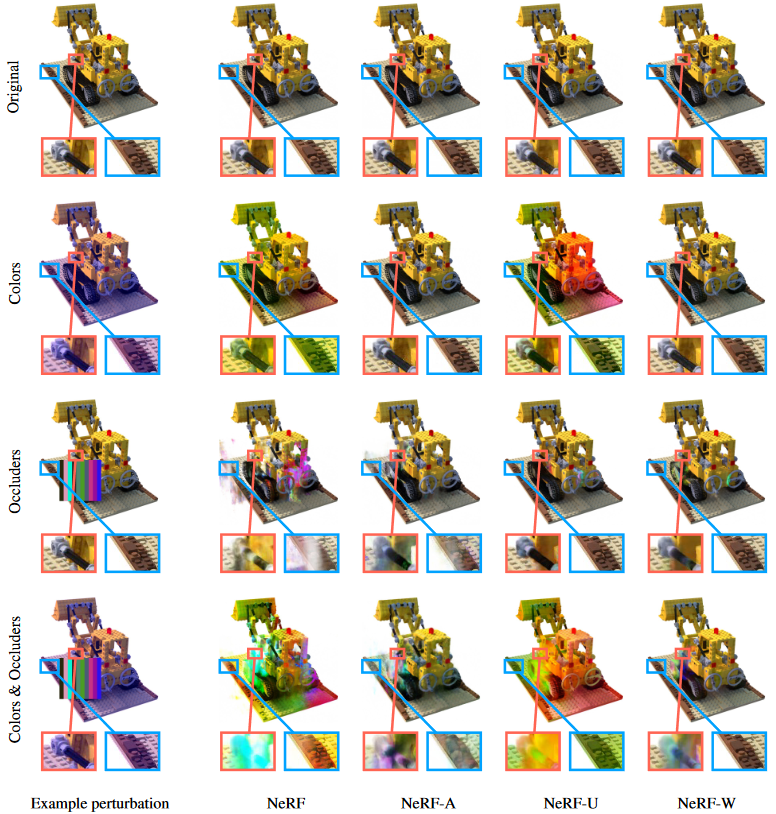
\includegraphics[width=.51\textwidth]{results-lego.png}
    \end{center}
\end{frame}

\begin{frame}{Concluding remarks}
    \begin{itemize}
        \item NeRF-W builds up on NeRF:
        \begin{itemize}
            \item disentangles 3D geometry and appearance embedding
            \item allows smooth interpolation between static geometry and appearance
            \item disentangles static representation and transient representation
            \item even more impressive results!
        \end{itemize}
        \bigskip
        \pause
        \item ... but still, it retains some NeRF limitations:
        \begin{itemize}
            \item ridicoulosly slow training time: 2~4 days for a scene!
            \item slow inference time, order of minutes
            \item oblique and rarely seen parts of images get blurry renderings
        \end{itemize}
    \end{itemize}
\end{frame}

\section{Our contribution}

\subsection{Tweaking complexity}
\begin{frame}{Tweaking complexity: faster train}
        \bold{Meta-learning}
        \begin{itemize}
            \item NeRF-W is a very dense network
            \item we can use meta-learning algorithms to learn better initialization
            \pause
            \item MAML and Reptile algorithms can be easily integrated\footnote{Tancik et al. 2020, \emph{Learned Initializations for Optimizing Coordinate-Based Neural Representations}, \url{https://arxiv.org/abs/2012.02189}}
            \pause
            \item consider \(\ell_i^{(\tau)}\)
            \begin{itemize}
                \item occluders patters are often predictables
                \item initialization does matter
            \end{itemize}
            \pause
            \item we can do better: we can meta-learn hyperparameters!\footnote{Baik et al. 2020, Meta-Learning with Adaptive Hyperparameters, \url{https://arxiv.org/abs/2011.00209v2}}
        \end{itemize}
\end{frame}

\begin{frame}{Tweaking complexity: faster inference}
    \bold{Network trimming}\footnote{Hu et al. 2016, \emph{Network Trimming: A Data-Driven Neuron Pruning Approach towards Efficient Deep Architectures},  \url{https://arxiv.org/abs/1607.03250v1}}
    \begin{itemize}
        \item APoZ: percentage of zero activations after ReLU
        \pause
        \item empirical result: many (631) in VGG-16 have APoZ \(>\) 90\%
        \bigskip
        \begin{figure}
            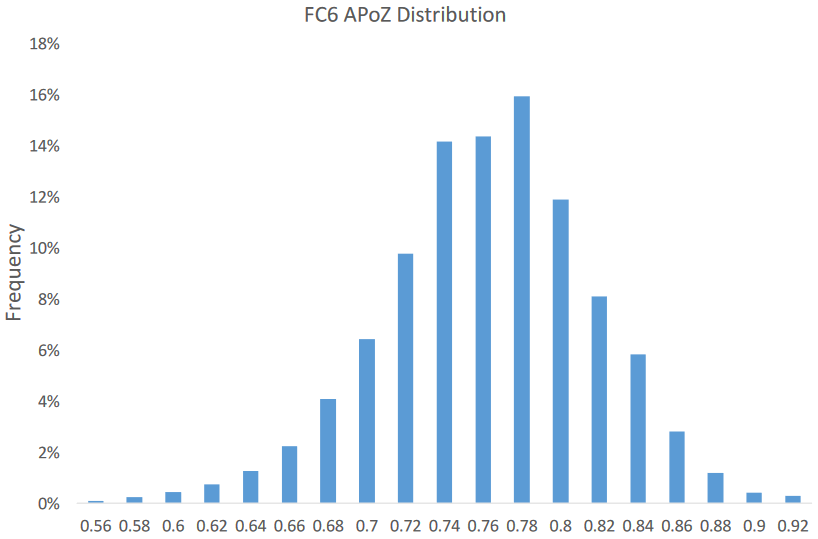
\includegraphics[width=.4\textwidth]{apoz.png}
        \end{figure}
    \end{itemize}
\end{frame}

\begin{frame}{Tweaking complexity: faster inference}
    \begin{itemize}
        \item High APoZ means that nodes provide little contribution to the output
        \begin{itemize}
            \item they can be pruned without affecting the result
            \item accuracy was even higher in some experiments!
        \end{itemize}
        \bigskip
        \pause
        \begin{figure}
            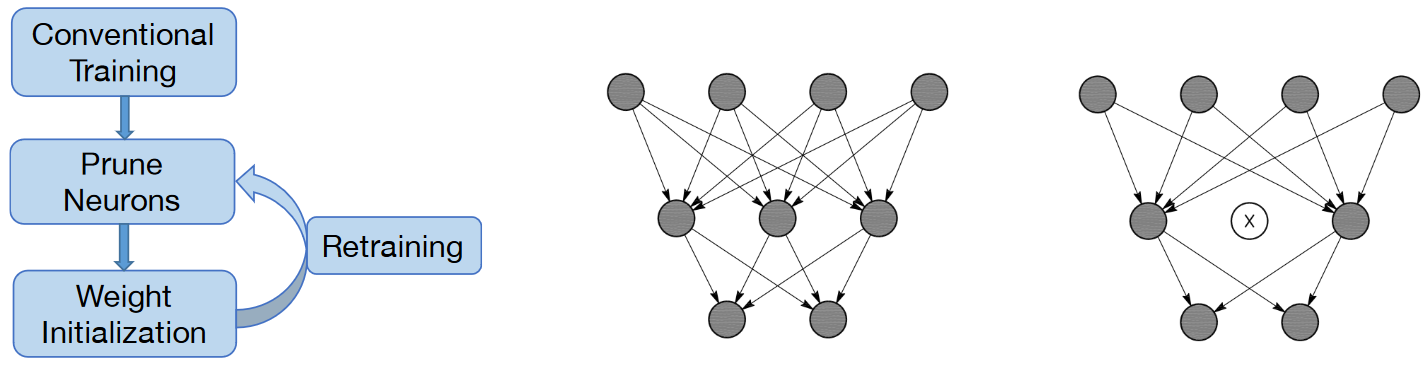
\includegraphics[width=.75\textwidth]{retrain.png}
        \end{figure}
        \bigskip
        \pause
        \item NeRF-W is a dense model
        \begin{itemize}
            \item fair to assume that there is redundancy
            \item pruning useless nodes does not affect results
            \item faster inference!
        \end{itemize}
    \end{itemize}
\end{frame}

\begin{frame}{SOTA review}
    Lots of interest and papers on NeRF efficiency!\footnote{Dellaert et Yen-Chen 2021, \emph{Neural volume rendering: NeRF and beyon}, \url{https://arxiv.org/abs/2101.05204v2}}
    \bigskip
    \begin{itemize}
        \item JaxNeRF
        \item AutoInt
        \item Learned initialization
        \item DeRF
        \item NeRF++
        \item Neural Sparse Voxel Fields
    \end{itemize}
\end{frame}

\subsection{Temporal latent embedding vector}
\begin{frame}{Temporal latent embedding vector}
    Extend NeRF-W to model simple dynamic scenes with GLO 
    \bigskip
    \pause
    \begin{figure}
        % \animategraphics[loop,autoplay,width=.35\textwidth]{20}{assets/gifs/waving-flag/waving-flag-}{0}{57}
    \end{figure}
    \pause
    \begin{itemize}
        \item pick a video, sample enough frames to describe the motion
        \item pick a time embedding vector \(\ell_i^{(\chi)}\) 
        \item make static density image dependent
        \item larger \(n^{(\chi)}\) accounts for more complex dynamic scenes 
    \end{itemize}
    \bigskip
    \begin{equation*}
        [\sigma_i(t), \vb{z}_i(t)] = \textrm{MLP}_{\theta_1} (\gamma_{\vb{x}}(\vb{x}), \alert{\ell_i^{(\chi)}})
    \end{equation*}    
\end{frame}

\begin{frame}{Proposal: NeRF-WT}
    \begin{onlyenv}<1>
        \begin{figure}
            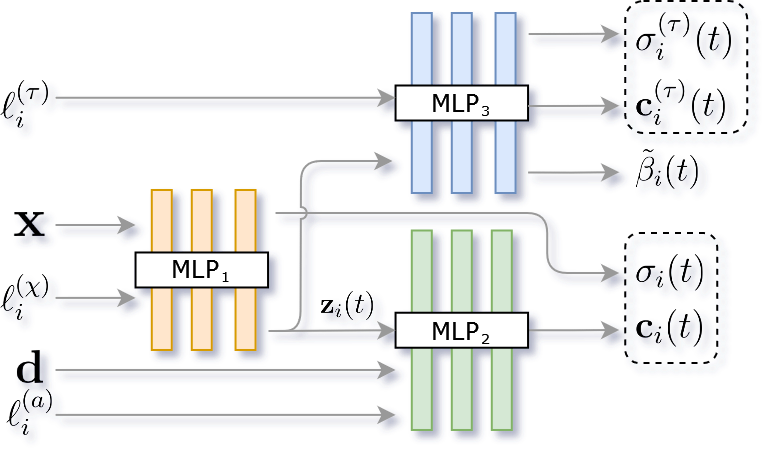
\includegraphics[width=.7\textwidth]{nerfwt-architecture.png}
        \end{figure}
    \end{onlyenv}
    \begin{onlyenv}<2>
        \begin{figure}
            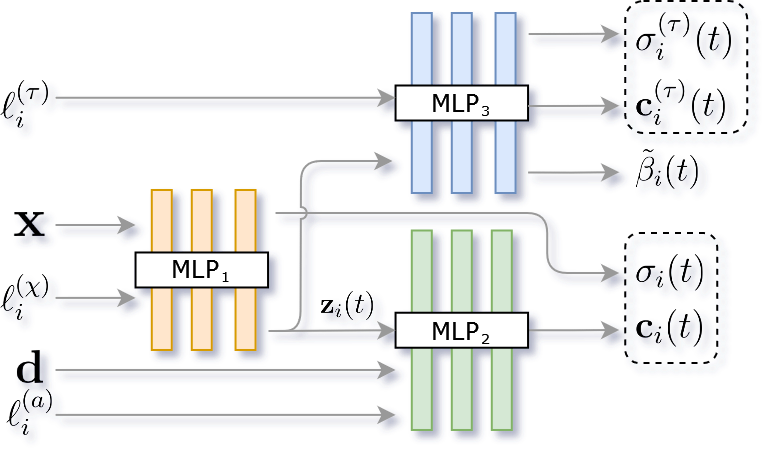
\includegraphics[width=.4\textwidth]{nerfwt-architecture.png}
        \end{figure}
        Some catches:
        \begin{itemize}
            \item consistency of static geometry
            \begin{itemize}
                \item use \(\ell_i^{(\chi)}\) only on fine models
                \item assumption: motion is simple enough and reasonably local
            \end{itemize}
            \item ambiguity on \(\ell_i^{(\chi)}\) and \(\ell_i^{(\tau)}\)
            \begin{itemize}
                \item "it may be not that bad of an issue"
            \end{itemize}
        \end{itemize}
    \end{onlyenv}
\end{frame}

\begin{frame}{Quick reminder}
    2021 was decades ago!
    \begin{figure}
        % \animategraphics[loop,autoplay,width=.61\textwidth]{60}{assets/gifs/block-nerf/block-nerf-}{0}{199}
    \end{figure}
\end{frame}

\begin{frame}[plain,noframenumbering]
    \begin{center}
        Thanks for your attention
    \end{center}
\end{frame}

\end{document}